%% LyX 2.1.3 created this file.  For more info, see http://www.lyx.org/.
%% Do not edit unless you really know what you are doing.
\documentclass[11pt]{article}
\usepackage[latin9]{inputenc}
\usepackage{geometry}
\geometry{verbose}
\usepackage{fancyhdr}
\pagestyle{fancy}
\usepackage{amsmath}
\usepackage{amssymb}
\usepackage{graphicx}

\makeatletter
%%%%%%%%%%%%%%%%%%%%%%%%%%%%%% User specified LaTeX commands.
\usepackage[margin=0.75in]{geometry} % see geometry.pdf on how to lay out the page. There's lots.
\usepackage{graphicx}
\usepackage{cleveref}
\usepackage{amsmath}
\usepackage{multirow}
\usepackage{listings}
\usepackage{color}
\usepackage{CJK}
\definecolor{mygreen}{RGB}{28,172,0}
\definecolor{mylilas}{RGB}{170,55,241}

\usepackage[latin9]{inputenc}
\usepackage{geometry}
\geometry{verbose}


\makeatletter
\@ifundefined{date}{}{\date{}}
\makeatother

%Fancy-header package to modify header/page numbering 
\usepackage{fancyhdr}
\pagestyle{fancy}
\lhead{\textbf{Ge/ESE 118}} %name of the course
\chead{\textbf{}} %topic of the homework set
\rhead{\textbf{Solution 7}} %number of the homework set
\lfoot{}
\cfoot{}
\rfoot{\thepage}


% Matlab script
\lstset{language=Matlab,%
      %basicstyle=\color{red},
  breaklines=true,%
  morekeywords={matlab2tikz},
  keywordstyle=\color{blue},%
  morekeywords=[2]{1}, keywordstyle=[2]{\color{black}},
  identifierstyle=\color{black},%}
  stringstyle=\color{mylilas},
  commentstyle=\color{mygreen},%
  showstringspaces=false,%without this there will be a symbol in the places where there is a space
  numbers=left,%
  numberstyle={\tiny \color{black}},% size of the numbers
  numbersep=9pt, % this defines how far the numbers are from the text
  emph=[1]{for,end,break},emphstyle=[1]\color{red}, %some words to emphasise
                                                      %emph=[2]{word1,word2}, emphstyle=[2]{style},    
}

\makeatother

\begin{document}

\subsection*{Problem 1 (graded by Kangchen) 30 points}


\subsubsection*{(a)- 5 points}

if $[\boldsymbol{U},\boldsymbol{S},\boldsymbol{V}]=svd(\boldsymbol{G})$,
so $\boldsymbol{G}=\boldsymbol{U}\boldsymbol{S}\boldsymbol{V}^{T}$,
thus $\boldsymbol{G}_{g}^{-1}=\boldsymbol{V}\boldsymbol{S}^{-1}\boldsymbol{U}^{T}$.
Note $S_{i,i}^{-1}=1/S_{i,i}$ for $S_{i,i}\neq0$, and $S_{i,i}^{-1}=0$
for $S_{i,i}=0$. The result is 
\begin{verbatim}
R1 =
    0.2839    0.4645    0.1484    0.1032
   -0.0194   -0.1226    0.0581    0.0839
R2 =
    0.2769    0.2154    0.3231    0.1846
   -0.3590    0.4615   -0.9744    0.8718
R3 =
    2.2194   12.7226   -5.6581   -8.2839
   -0.0194   -0.1226    0.0581    0.0839
R4 =
    0.0250    0.0250    0.0250    0.0250
    0.0750    0.0750    0.0750    0.0750
\end{verbatim}
\selectlanguage{english}%

\subsubsection*{(b)- 5 points}

$\boldsymbol{G}_{LLS}^{-1}=inv(\boldsymbol{G}^{T}\boldsymbol{G})\boldsymbol{G}^{T}$.
But if $\det{\boldsymbol{G}^{T}\boldsymbol{G}}=0$, then the least
square problem will have infinitely many solutions that gives the
same minimized error, which means $\boldsymbol{G}_{LLS}^{-1}$ is
not well defined in this case. 
\begin{verbatim}
L1 =
    0.2839    0.4645    0.1484    0.1032
   -0.0194   -0.1226    0.0581    0.0839
L2 =
    0.2769    0.2154    0.3231    0.1846
   -0.3590    0.4615   -0.9744    0.8718
L3 =
    2.2194   12.7226   -5.6581   -8.2839
   -0.0194   -0.1226    0.0581    0.0839
L4 =
   Inf   Inf   Inf   Inf
   Inf   Inf   Inf   Inf
\end{verbatim}
\selectlanguage{english}%

\subsubsection*{\tiny
\lstinputlisting{./hw7p1.m}
\normalsize}


\subsubsection*{(c)- 5 points}

When least square inverse is unique, $\det{\boldsymbol{G}^{T}\mathbf{G}}\neq0$,
$\boldsymbol{G}_{LLS}^{-1}$ is the same as general inverse, because
\begin{eqnarray*}
\boldsymbol{G} & = & \boldsymbol{US}\boldsymbol{V}^{T}\\
\boldsymbol{G}^{T} & = & \boldsymbol{V}\boldsymbol{S}^{T}\boldsymbol{U}^{T}\\
\boldsymbol{G}^{T}\boldsymbol{G} & = & \boldsymbol{V}(\boldsymbol{S}^{T}\boldsymbol{S})\boldsymbol{V}^{T}\\
(\boldsymbol{G}^{T}\boldsymbol{G})^{-1} & = & \boldsymbol{V}(\boldsymbol{S}^{T}\boldsymbol{S})^{-1}\boldsymbol{V}^{T}\\
(\boldsymbol{G}^{T}\boldsymbol{G})^{-1}\boldsymbol{G}^{T} & = & \boldsymbol{V}(\boldsymbol{S}^{T}\boldsymbol{S})^{-1}\boldsymbol{S}^{T}\boldsymbol{U}^{T}\\
 & = & \boldsymbol{V}\boldsymbol{S}^{-1}\boldsymbol{U}^{T}\\
 & = & \boldsymbol{G}_{g}^{-1}
\end{eqnarray*}
which is the same as generalized inverse. Note in the above derivation,
$U$,$V$ is square orthgonal matrix, where $\boldsymbol{S}$, $\boldsymbol{S}^{-1}$
is diagnoal but not square matrix, and $\boldsymbol{S}^{T}\boldsymbol{S}$
has inverse.

When $\det{\boldsymbol{G}^{T}\boldsymbol{G}}=0$ , $\boldsymbol{G}_{LLS}^{-1}$
is not well defined, and general inverse gives the solution that satisfies
least square problem and at the same time minimizes the L2 norm of
the model.


\subsubsection*{(d)- 5 points}

Note that $\boldsymbol{G}_{g}^{-1}\boldsymbol{d}$ gives the estimation
of intercept and slope of the 4 points least square problem, whose
$\boldsymbol{X}$ is given by second column of $\mathbf{G}$. This
explains why $\mathbf{G}_{1g}^{-1}$ has the same second row as $\mathbf{G}_{3g}^{-1}$,
because \textbf{$\mathbf{X}$} in $\mathbf{G}_{3}$ is just a shift
of $\mathbf{X}$ in $\mathbf{G}_{1}$.

For $\mathbf{G}_{1},\mathbf{G}_{2},\mathbf{G}_{3}$, the two columns
are linearly independent, so they have full column rank, then 
\begin{eqnarray*}
\mathbf{G}_{g}^{-1}\mathbf{G} & = & \mathbf{V}\mathbf{S}^{-1}\mathbf{U}^{T}\mathbf{U}\mathbf{S}\mathbf{V}^{T}\\
 & = & \mathbf{V}\mathbf{S}^{-1}\mathbf{S}\mathbf{V}^{T}\\
 & = & \mathbf{V}\mathbf{V}^{T}\\
 & = & \mathbf{I}
\end{eqnarray*}
So the 1st row of $\mathbf{G}_{g}^{-1}$ dot product with 1st column
of $\mathbf{G}$ will be 1, the 2nd row of $\mathbf{G}_{g}^{-1}$
dot product with 2nd column of $\mathbf{G}$ will be 1, and the 1st
row of $\mathbf{G}_{g}^{-1}$ dot product with 2nd column of $\mathbf{G}$
will be 0, the 2nd row of $\mathbf{G}_{g}^{-1}$ dot product with
1st column of $\mathbf{G}$ will be 0. This explains roughly, for
example, the relative higher amplitude of the first row of $\mathbf{G}_{3}^{-1}$
compared with the 2nd row of $\mathbf{G}_{3}^{-1}$. However, we must
be careful about such amplitude comparison, because for example the
2nd row of $\mathbf{G}_{1}^{-1}$ and the 2nd row of $\mathbf{G}_{3}^{-1}$
is the same, although amplitude in $\mathbf{G}_{1}$ and $\mathbf{G}_{3}$
is quite different.

For $\mathbf{G}_{4}$, whose rank is 1, note that the least square
solution will require $m_{1}+3m_{2}=const$. This is a line in $m_{1}~m_{2}$
plane. The L2 norm of the model, will corresponding to a line segment
from origin to this line, which got minimized when it's perpendicular
to this line, or $m_{1}/m_{2}=1/3$. This explains why $\mathbf{G}_{4}^{-1}$,
also a rank 1 matrix, has two rows whose amplitude ratio is 1/3.


\subsection*{Problem 2 (graded by Yiran) 38 points}


\subsubsection*{(a)- 5 points}

Looking at the SVDs of the G matrices from problem 1, we see a couple
inverses that would potentially benefit from a truncated SVD. Truncation
is a useful strategy when there is a large disparity between sizes
of singular values. We don't care about the absolute value of the
singular values (unless they are close to machine precision $(~10^{-16})$),
we only care about the relative size of the singular values to one
another. The first 3 G matrices each have two singular values, so
we can take the ratio of these two values to see which matrices might
require truncation. G4 only has 1 nonzero singular value, so it is
effictively already truncated. If we look at the ratios of singular
values $\frac{s_{2}}{s_{1}}$ we get:

\begin{equation}
\mathbf{G}1:\frac{s_{2}}{s_{1}}=0.2393
\end{equation}


\begin{equation}
\mathbf{G}2:\frac{s_{2}}{s_{1}}=0.3469
\end{equation}


\begin{equation}
\mathbf{G}3:\frac{s_{2}}{s_{1}}=3.000*10^{-4}
\end{equation}


G3 has the smallest ratio by several orders of magnitude, so it is
out best candidate for truncation. G1 has a smaller ratio than G2,
so it would be our second most amenable matrix for truncation.

Truncation has the advantage of removing errors potentially caused
by small singular values; thus, not allowing these errors to propagate
through the rest of our calculations. However, the disadvantage here
is that we are removing information and often the smallest singular
values also contain the most information. We want to use truncation
in order to keep the most amount of information that isn't dominated
by errors or noise.


\subsubsection*{(b)- 5 points}

We select G3 as the most amenable to a truncated SVD. The recalculation
yields:

\begin{equation}
\mathbf{G}3_{GeneralizedInverseTruncated}=\begin{pmatrix}0.0000 & 0.0000 & 0.0000 & 0.0000\\
0.0024 & 0.0023 & 0.0025 & 0.0025
\end{pmatrix}
\end{equation}



\subsubsection*{(c)- 5 points}

The second most amenable matrix is G1. The recalculation

\begin{equation}
\mathbf{G}3_{GeneralizedInverseTruncated}=\begin{pmatrix}0.0031 & -0.0078 & 0.0114 & 0.0141\\
0.0216 & -0.0537 & 0.0780 & 0.0969
\end{pmatrix}
\end{equation}



\subsubsection*{\tiny
\lstinputlisting{./hw7p2.m}
\normalsize}


\subsubsection*{(d)- 5 points}

We calculate the generalized inverse model solutions using both the
original SVD and the truncated versions for both G1 and G3 for each
of the datasets $d_{1}$ and $d_{2}$. The plots are attached below.
Here are the solutions:
\begin{verbatim}
m1d1 =

   10.5226
   -0.0129


m1d2 =

   10.4652
   -0.2658


m3d1 =

   11.8129
   -0.0129


m3d2 =

   37.0458
   -0.2658


mt1d1 =

    0.2171
    1.4893


mt1d2 =

    0.1798
    1.2335


mt3d1 =

    0.0010
    0.1031


mt3d2 =

    0.0010
    0.0979
\end{verbatim}
\selectlanguage{english}%
\begin{figure}
\centering{}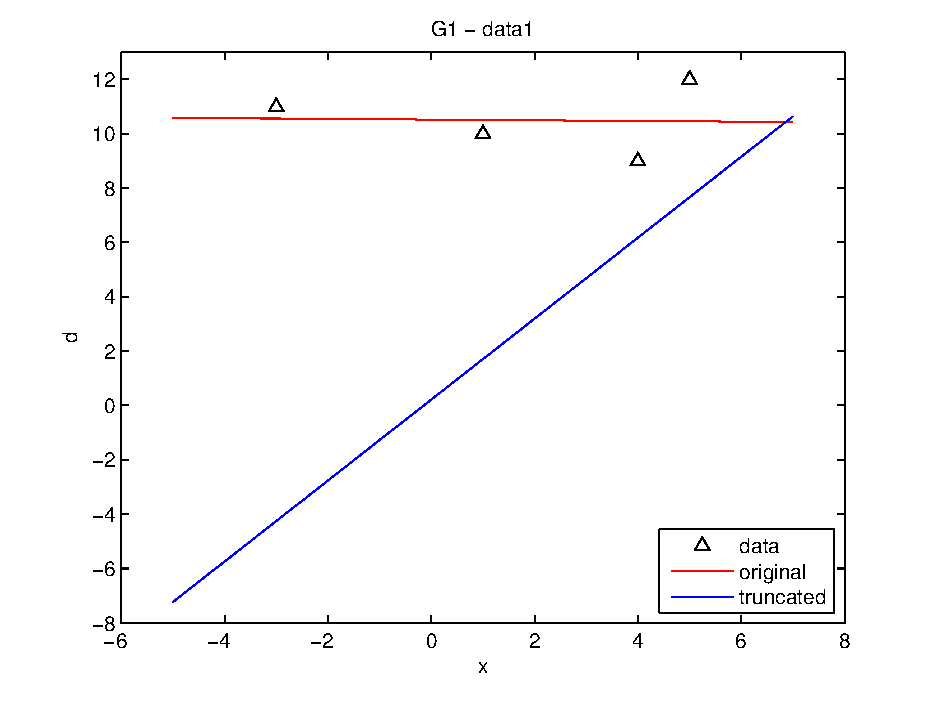
\includegraphics[width=12cm]{p2fig1} 
\end{figure}


\begin{figure}
\centering{}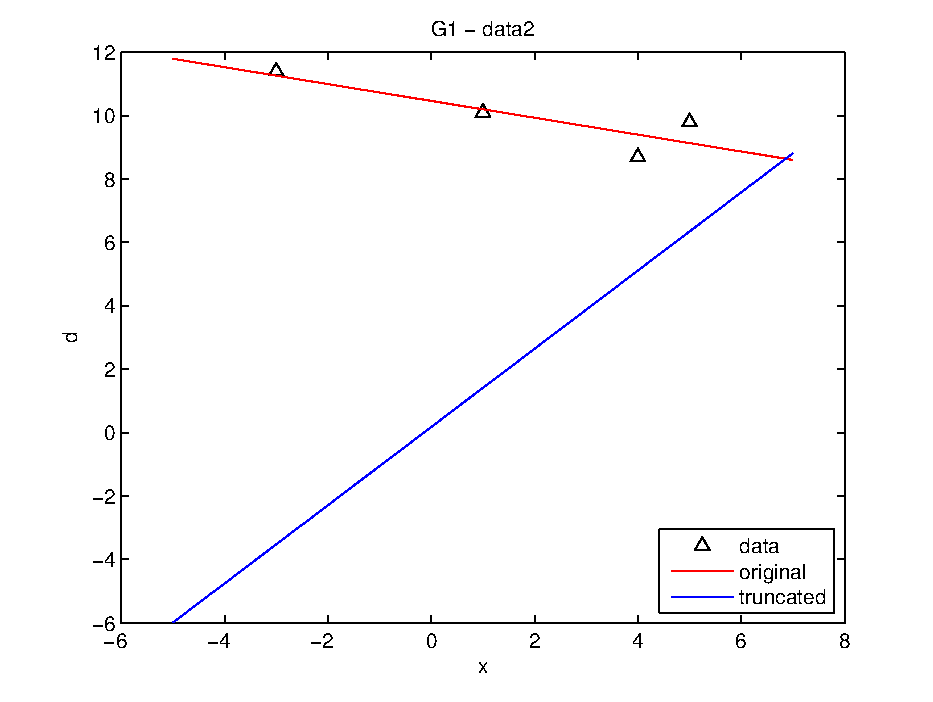
\includegraphics[width=12cm]{p2fig2} 
\end{figure}


\begin{figure}
\centering{}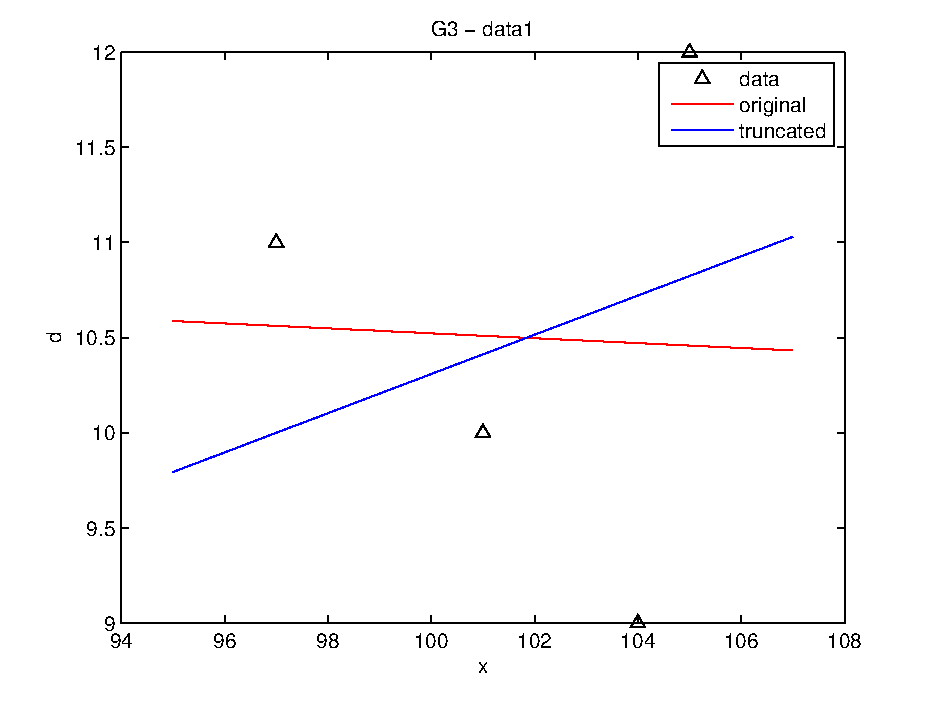
\includegraphics[width=12cm]{p2fig3} 
\end{figure}


\begin{figure}
\centering{}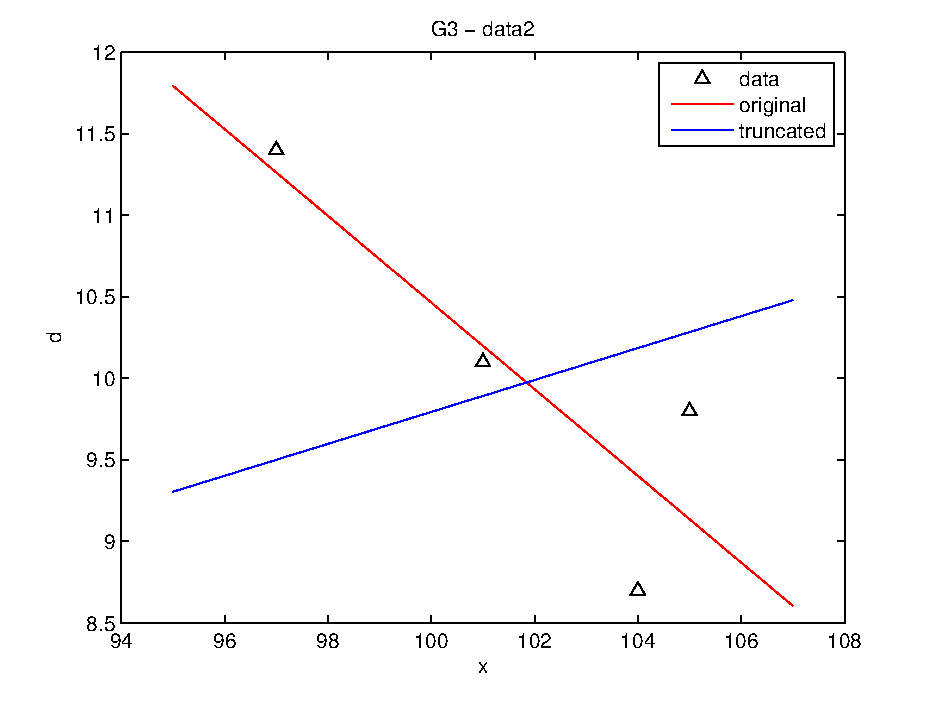
\includegraphics[width=12cm]{p2fig4} 
\end{figure}



\subsubsection*{(e)- 5 points}

Looking at the plots we can see a large difference between the original
and the truncated cases. We have truncated the smallest singular value,
which influences both rows of the generalized inverse. However, it
more significantly influences the first row, which controls our model
parameter $m_{1}$ (the y-intercept). If we look at our original models,
most seem to fit the data reasonably (as reasonably as a line can
fit) and all have a negative slope. Our truncated models all have
positive slopes and many don't seem to explain the data well at all.
This is because our truncation eliminated any information about y-intercept,
and thus all the models have y-intercepts of 0 no matter what the
data. We can see this behavior clearly on the y-intercept on Toby's
plots in the solution for problem 3. As far as which models we would
prefer, it would depend on what we know about the dataset. In all
cases besides G3-data 1 we would likely prefer the original models
because they seem to fit the data better, unless we had some prior
information about the y-intercept. For the G3-data 1 neither model
seems to fit very well, so it may be better to prefer the truncated
model as it is more likely to avoid errors.


\subsection*{Problem 3 (graded by Toby) 32 points}


\subsubsection*{(a)- 5 points}

The MATLAB code that generates the matrices is attached at the end
of this section. The matrices are calculated using $m=(G^{T}G+\alpha^{2}I)^{-1}G^{T}d$.
The matrices are \begin{subequations} 
\begin{align*}
\mathbf{G}_{1,g,T,\alpha_{1}}^{-1} & =\begin{pmatrix}0.282931351378109 & 0.462937664456661 & 0.147926616569195 & 0.102925038299558\\
-0.019222102718031 & -0.122340004924458 & 0.058116323936789 & 0.083895799488396
\end{pmatrix}\\
\mathbf{G}_{2,g,T,\alpha_{1}}^{-1} & =\begin{pmatrix}0.275661587810746 & 0.215517241379310 & 0.320769847634322 & 0.185445068163593\\
-0.351343223736969 & 0.452586206896552 & -0.954290296712109 & 0.854550922213312
\end{pmatrix}\\
\mathbf{G}_{3,g,T,\alpha_{1}}^{-1} & =\begin{pmatrix}0.604003054340609 & 3.462399532543330 & -1.539794304311428 & -2.254393423862098\\
-0.003493985867091 & -0.031656565418916 & 0.017627948796778 & 0.024668593684735
\end{pmatrix}\\
\mathbf{G}_{4,g,T,\alpha_{1}}^{-1} & =\begin{pmatrix}0.024993751562093 & 0.024993751562093 & 0.024993751562093 & 0.024993751562093\\
0.074981254686328 & 0.074981254686328 & 0.074981254686328 & 0.074981254686328
\end{pmatrix}\\
\mathbf{G}_{1,g,T,\alpha_{2}}^{-1} & =\begin{pmatrix}0.262125138837468 & 0.427989633469086 & 0.137726767863754 & 0.096260644205850\\
-0.016290262865605 & -0.116993706034802 & 0.059237319511292 & 0.084413180303591
\end{pmatrix}\\
\mathbf{G}_{2,g,T,\alpha_{2}}^{-1} & =\begin{pmatrix}0.251592356687898 & 0.213375796178344 & 0.280254777070064 & 0.194267515923567\\
-0.230891719745223 & 0.310509554140127 & -0.636942675159236 & 0.581210191082802
\end{pmatrix}\\
\mathbf{G}_{3,g,T,\alpha_{2}}^{-1} & =\begin{pmatrix}0.032727078270480 & 0.187497400490787 & -0.083350663394751 & -0.122043243949828\\
0.002115257782188 & 0.000499105768831 & 0.003327371792206 & 0.003731409795545
\end{pmatrix}\\
\mathbf{G}_{4,g,T,\alpha_{2}}^{-1} & =\begin{pmatrix}0.024844720496894 & 0.024844720496894 & 0.024844720496894 & 0.024844720496894\\
0.074534161490683 & 0.074534161490683 & 0.074534161490683 & 0.074534161490683
\end{pmatrix}
\end{align*}
\end{subequations}


\subsubsection*{(b)- 5 points}

For the generalized inverse we have that 
\begin{equation}
\mathbf{G}_{g}^{-1}=\sum_{i=1}^{p}\frac{s_{i}^{2}}{s_{i}^{2}+\alpha^{2}}\frac{1}{s_{i}}v_{i}u_{i}^{T},
\end{equation}
where $p$ is the index of the last nonzero singular value. For the
regularized inverse, we have extra factors in the expansion that introduce
a ``smooth'' truncation, i.e., for large $s_{i}$ the term is 1
and for small $s_{i}$ it is zero. This means that the similarity
between the truncated and regularized matrices is determined by the
relative size of the singular values compared to $\alpha$. For $G_{1}$,
$G_{2}$ the singular values are larger than the Tikhonov parameters,
implying that the truncated and regularized inverses should look different.
For $\mathbf{G}_{3}$ we have that $s_{1}^{2}>>\alpha_{1}^{2},\alpha_{2}^{2}$,
$s_{2}^{2}\sim\alpha_{1}^{2}$ and $s_{2}^{2}<<\alpha_{2}^{2}$. According
to the equation above, this implies that the truncated and regularized
inverses are different for $\alpha=0.1$, but similar for $\alpha=0.5$.
For $\mathbf{G}_{4}$ the truncated and the regularized must be different,
because we only have two singular values, one of which is $0$ anyway.


\subsubsection*{(c)- 5 points}

The four plots are

\noindent Here is a plot of the profile: 
\begin{figure}
\centering{}\includegraphics[width=12cm]{p3b1} 
\end{figure}


\begin{figure}
\centering{}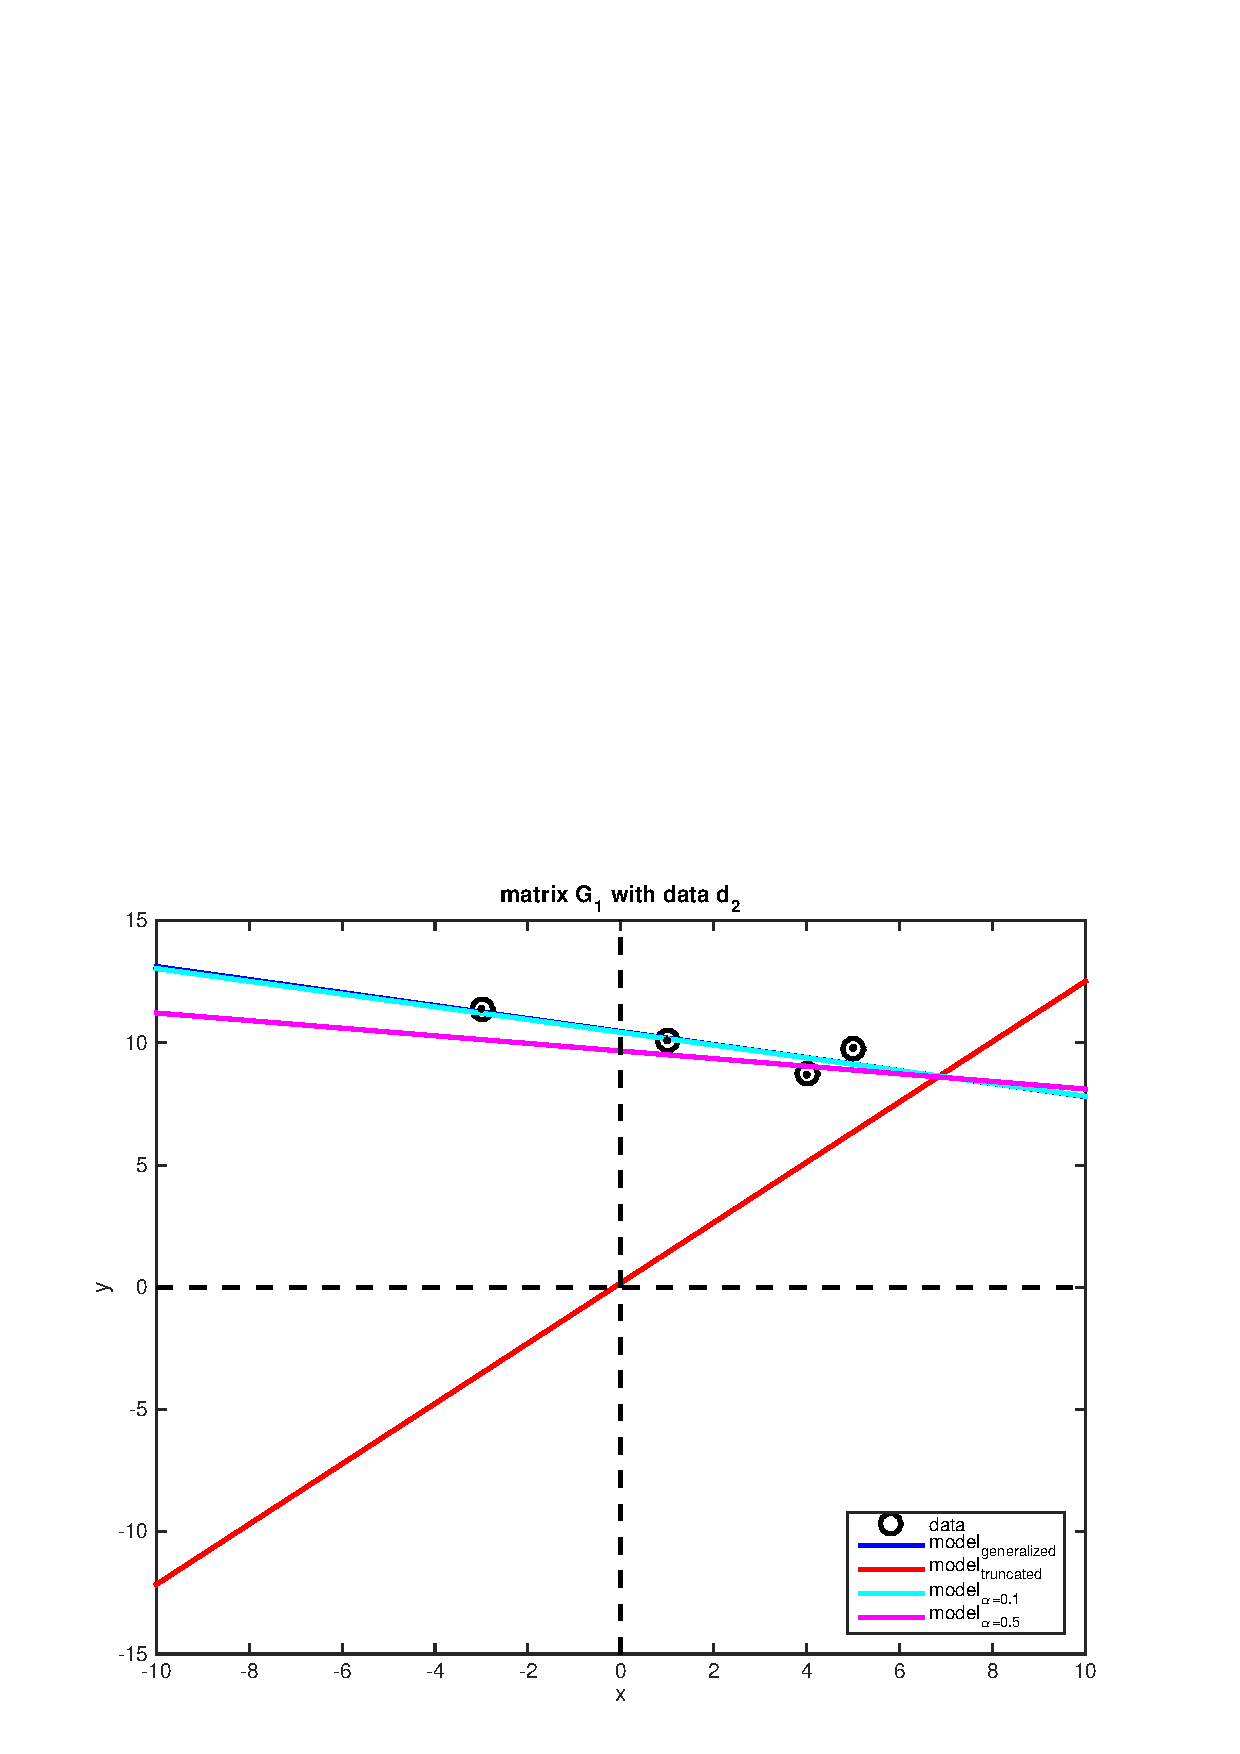
\includegraphics[width=12cm]{p3b2} 
\end{figure}


\begin{figure}
\centering{}\includegraphics[width=12cm]{p3b3} 
\end{figure}


\begin{figure}
\centering{}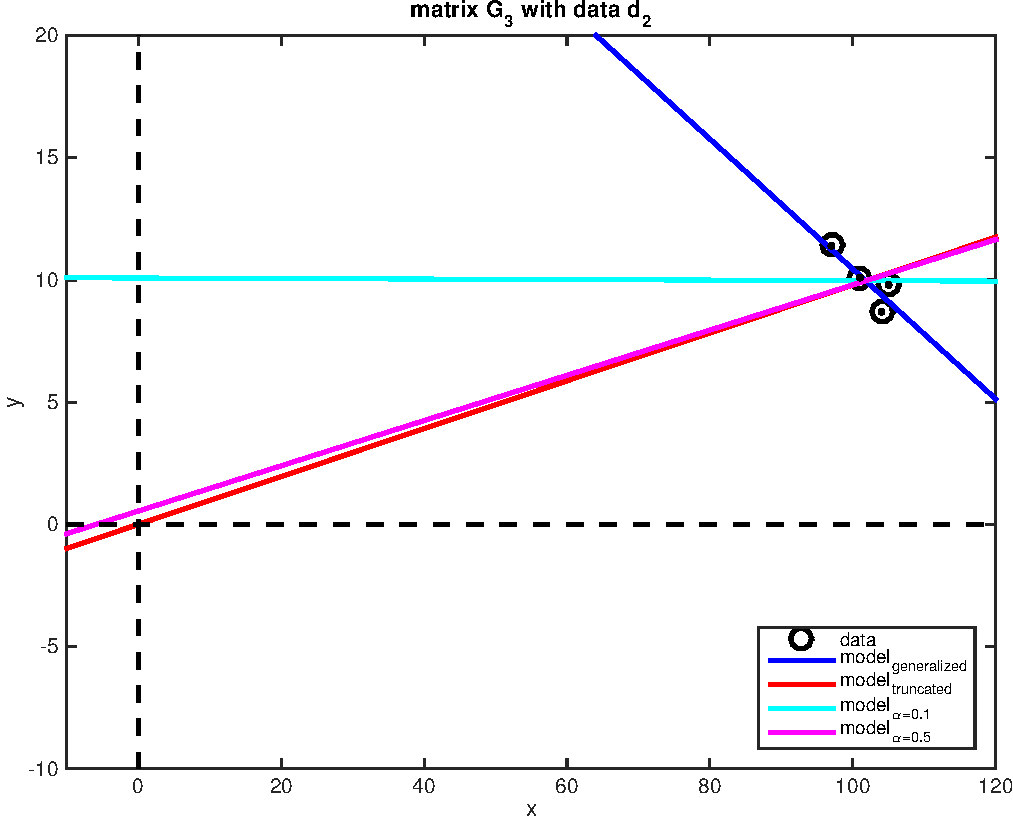
\includegraphics[width=12cm]{p3b4} 
\end{figure}



\subsubsection*{(d)- 5 points}

For $\mathbf{G}_{3}$ the truncated model and the Tikhonov model with
$\alpha=0.5$ are very close. This is because of a term $s_{i}^{2}/(s_{i}^{2}+\alpha^{2})$
in the expansision for the generalized inverse in terms of its singular
values is almost zero for the smallest singular value of $\mathbf{G}_{3}$
and almost $1$ for the largest singular value when $\alpha=0.5$.
Thus the truncated and the regularized models are very close. This
is not the case for $\mathbf{G}_{1}$, because the singular values
are not as far apart and always larger than $\alpha$, but not by
several orders of magnitude. Thus the truncated and the regularized
models are giving different answers. In fact, for small truncation
parameters, the regurlazied model is close to the generalized inverse
model.

\noindent MATLAB script:

\noindent \tiny
\lstinputlisting{./p3.m}
\normalsize
\end{document}
